% !TeX spellcheck = en_US
\section{Problem 8}
Adadelta is another variant of the AdaGrad algorithm. The main difference lies in the fact that it decreases the amount by which the learning rate is adaptive to coordinates. Moreover, traditionally it referred to as not having a learning rate since it uses the amount of change itself as calibration for future change. Adadelta is an extension to the Gradient Descent Optimization Algorithm. Although, it is better understood as an extension of the AdaGrad and RMSProp algorithms. \\

The idea was derived mainly from ADAGRAD in order to improve upon the two main drawbacks of the method.
\begin{enumerate}
	\item The continual decay of learning rates throughout training
	\item The need for a manually selected
	global learning rate
\end{enumerate}

All things considered, in this exercise we are given the following function:
\begin{equation}
	F(w) = 0.1w_1^2 + 2w_2^2
\end{equation}
\label{eq:Funcproblem8}
\vspace{1mm}

\subsection{Question A}
To find the minimum of the Function ~\ref{eq:Funcproblem8} using the AdaDelta optimizer, instead of the gradient descent, we need to iteratively update the weights $w_1$ and $w_2$ based on the optimizer's rules. ADADELTA is an adaptive learning rate optimization algorithm that adjust the learning rate during training. Adadelta computes a moving average of the parameter updates and the learning rate is adjusted based on this moving average.\\

The Adadelta algorithm has two main parameters: $\rho$ and $e$. We will set:
\begin{itemize}
	\item Decay rate $\rho = 0.9$
	\item Constant $\epsilon = 10^{-6}$ 
\end{itemize}

$\epsilon$ is a small value which is added to maintain numerical stability.\\
The $\rho$ variable is a hyperparameter that controls the decay rate of the running averages of the squared gradients, $\mathbf{s}_{t}$, and squared parameter updates,	$\Delta{\bf x}_{t}$.\\

Based on these values, we will briefly explain the algorithm of AdaDelta. In a nutshell, AdaDelta uses two state variables, $\bm{s_t}$ to store a leaky average of the second moment of the gradient and $\bm{\Delta x_t$} to store a leaky average of the second moment of the change of parameters in the model itself.\\

Given the parameter $\rho$, we obtain the following leaky updates:
\begin{equation}
	\mathbf{s}_{t}=\rho\mathbf{s}_{t-1}+(1-\rho)\mathbf{g}_{t}^{2}
\end{equation} 
A crucial point and difference from the RMSProp algorithm is that we perform updates with the rescaled gradient $\bm{g_t'}$. So, each time the weights are updated as:
\begin{equation}
	\mathbf{w}_{t}=\mathbf{w}_{t-1}-\mathbf{g}_{t}^{\prime}.
\end{equation}

where the rescaled gradient is calculated as:
\begin{equation}
	\mathbf{g}_{t}^{\prime}={\frac{\sqrt{\Delta\mathbf{x}_{t-1}+\epsilon}}{\sqrt{\mathbf{s}_{t}+\epsilon}}}~\mathbf{g}_{t}
\end{equation}

Here, $\bm{\Delta x_{t-1}}$ is the leaky average of the squared rescaled gradient $\mathbf{g}_{t}^{\prime}$. We initialize $\bm{\Delta x_{0} = 0}$ and update each step with ${g}_{t}^{\prime}$ as this equation shows:

\begin{equation}
	\Delta{\bf x}_{t}=\rho\Delta{\bf x}_{t-1}+(1-\rho){\bf g}_{t}^{\prime2},
\end{equation}

For a better understanding of the topic, we will provide a pseudo-code of the ADADELTA algorithm.
	\begin{algorithm}[H]
		\caption{Computing ADADELTA update at time $t$}
		\begin{algorithmic}
			\Require Decay rate $\rho$, Constant $\epsilon$, Learning rate $\alpha$
			\Require Initial parameter $x_1$
			\State Initialize accumulation variables $S_t\_0 = 0$, $\Delta x_t\_0 = 0$
			\For{$t = 1$ \textbf{to} $T$} 
			\State Compute Gradient: $g_t$
			\State Accumulate Gradient: $S_t = \rho S_{t-1} + (1 - \rho)g_t^2$
			\State Compute Update: $	\mathbf{g}_{t}^{\prime}={\frac{\sqrt{\Delta\mathbf{x}_{t-1}+\epsilon}}{\sqrt{\mathbf{s}_{t}+\epsilon}}}~\mathbf{g}_{t}$
			\State Accumulate Updates: 	$\Delta{\bf x}_{t}=\rho\Delta{\bf x}_{t-1}+(1-\rho){\bf g}_{t}^{\prime2}$
			\State Apply Update: $x_{t+1} = x_t - (a*g_{t}^{\prime})$
			\EndFor
		\end{algorithmic}
	\end{algorithm}
it is very important to emphasize on the tricky part of the provided pseudo-code, because we have slightly changed it. For this exercise we want to include the learning rate in our optimizer. However, as we mentioned before, AdaDelta is an optimizer that doesn't use a learning rate. Taking everything into account, we modified the traditional update
\begin{equation}
	{x}_{t+1}={x}_{t}-{g}_{t}^{\prime}.
\end{equation}
into
\begin{equation}
	x_{t+1} = x_t - (a \cdot g_{t}^{\prime})
\end{equation}

To conclude, to point out the operation of the AdaDelta algorithm, we will plot the algorithm’s trajectory on a contour plot of F(x).
\begin{figure}[H]
	\centering
	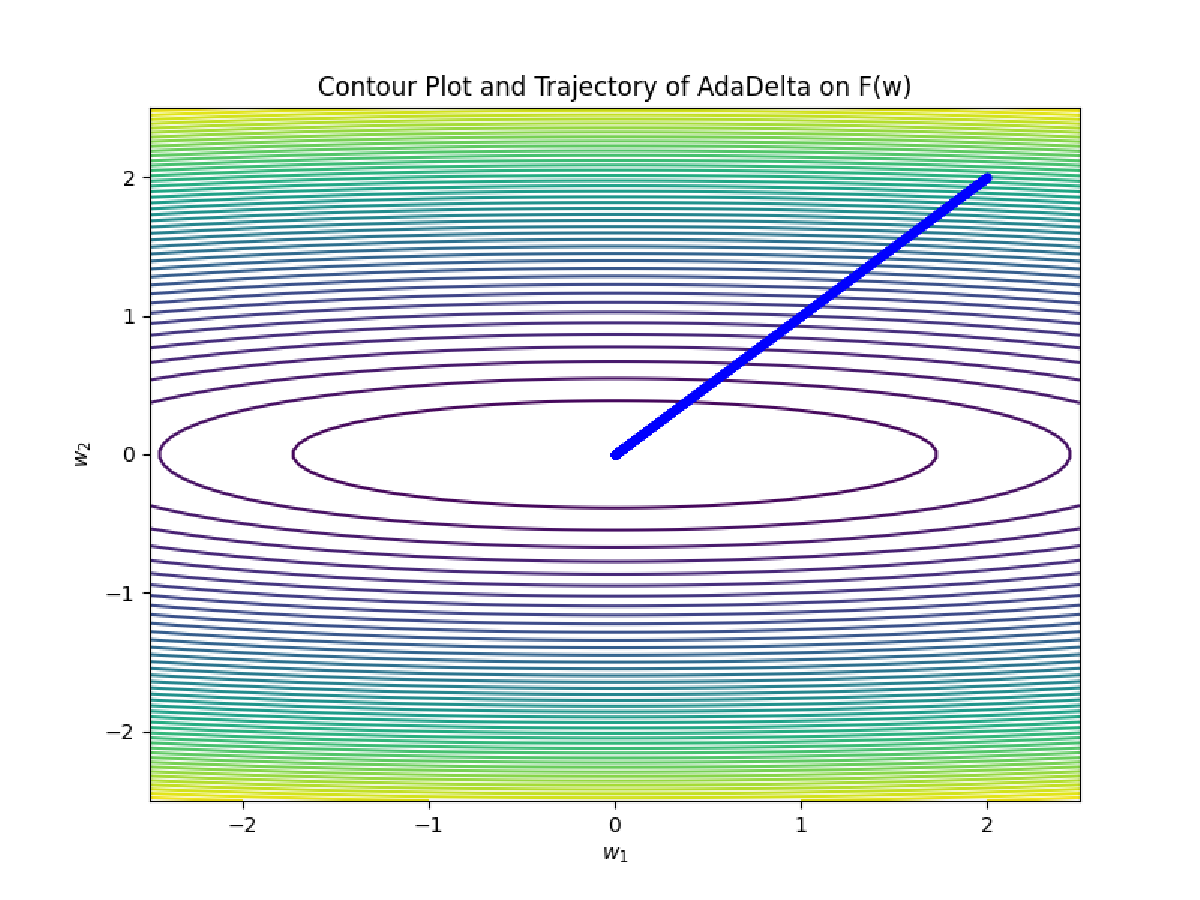
\includegraphics[width=.7\textwidth]{../Problem 8/ADADELTA_04.pdf}
	\caption{AdaDelta algorithm and trajectory with learning rate $\alpha=0.4$}
	\label{fig:lr=0.4}
\end{figure}
\vspace{2mm}

\subsection{Question B}
As previously mentioned, in the AdaDelta optimization algorithm, the learning rate is adaptively changed based on the running average of the recent gradients and the recent parameter updates. This is different from many other optimization algorithms where the learning rate is a fixed hyperparameter.\\
But, in this example we will show once again how by implementing some tricks we can still define it and observe how it can affect the algorithm's trajectory.\\

On the previous question, we plotted the algorithm's trajectory for learning rate $\alpha=0.4$. When we change it to $\alpha=3$ we can remark some crucial points.
\begin{figure}[H]
	\centering
	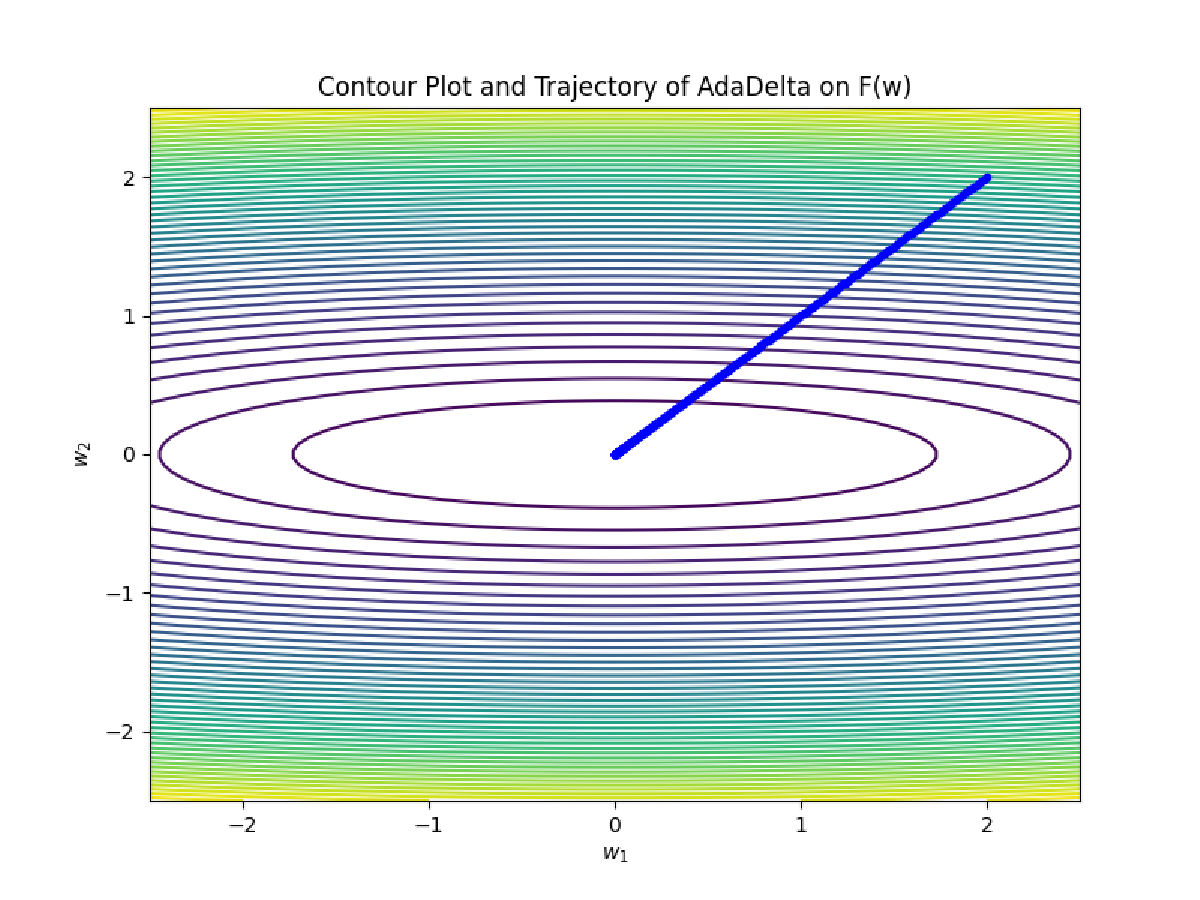
\includegraphics[width=.7\textwidth]{../Problem 8/ADADELTA_3.pdf}
	\caption{AdaDelta algorithm and trajectory with learning rate $\alpha=3$}
	\label{fig:lr=3}
\end{figure}
\vspace{2mm}

In drawing things to a close, based on Figure~\ref{fig:lr=0.4} and Figure~\ref{fig:lr=3} we can evaluate the impact of the learning rate and to take a closer look on the algorithm.\\

In both plots, the contours represent levels of the function $F(w)$ with each line indicating the points where the function has the same value. The closer the lines, the steeper the gradient at that point. The central region where the lines are more widely spaced indicates the minimum of the function.\\

The observation that we can highlight is the speed of convergence. A larger learning rate generally means that the optimizer makes larger steps in the parameter space. If the learning rate is set appropriately, this can lead to faster convergence to the minimum of the function. Though, there is a big risk of overshooting the minimum, which means that the optimizer could oscillate around the minimum, or in the worst case, to diverge.\\
Dissimilar to it, in Figure~\ref{fig:lr=3}, it appears that the AdaDelta optimizer with a higher learning rate has discovered a trajectory that approaches the function's central minimum more closely. This suggests that effective parameter space exploration has been made possible by the higher learning rate without leading to instability in the optimization procedure.\\
With the help of our code we discovered that for the same \textit{number of iterations = $2000$}, the optimizer with \underline{learning rate lr = 0.4} converges after \textbf{1236 iterations} at $\left[\num{1.21918e-05},\ \num{4.01599e-31}\right]$  and with \underline{learning rate lr = 3} after \textbf{315 iterations} at $\left[\num{2.37591e-06},\ \num{6.35476e-07}\right]$.
\vspace{2mm}

\subsection{Question C}
As a last note, we would like to test AdaDelata with the same objective function rotated by 45\degree. Hence, now we have the following objective function:
\begin{equation}
	F(w) = 0.1(w_1 + w_2)^2 + 2(w_1 - w_2)^2
\end{equation}
\label{eq:RotatedFuncproblem8}
\vspace{1mm}

We may export our final observations by comparing the code for the original function and the rotated one.\\

Similar to other gradient-based optimization techniques, the AdaDelta approach is invariant to orthogonal transformations like rotations. This is because orthogonal transformations maintain the angles and distances between vectors.Rotating an objective function by 45 degrees, or any other angle, in its variable space doesn't change the intrinsic properties of the function such as its minima, maxima, or saddle points.What changes is the coordinate system in which you are expressing the function.

To observe the behavior of the AdaDelta optimization algorithm on the rotated objective function, we can compare its convergence with the original objective function and see if they behave differently in terms of convergence. We notice that both objective functions ultimately converge to a similar minimum value with similar number of iterations, which suggests that the rotated function behaves simirarly to the original function in terms of convergence. \\

In addition to convergence behavior, we can notice other similarities and differences between the original and rotated function.\\
By geometry, the original function is an elliptical bowl with its major axis aligned with the coordinate axes, while the rotated one has a more circular or isotropic shape, as it combines $(w_1 + w_2)$ and $(w_1 - w_2)$ terms, resulting into a more balanced sensitivity to changes of $w_1$,$w_2$. The shape of the contour of the function will appear rotated by 45 \degree, but the relative distances between the contours will remain the same, which means the steepness or flatness of the function does not change.\\

By gradient behavior, the gradients of the original function have larger components in the $w_2$ direction due to the higher coefficient for $w_2^2$ . As a result, during optimization, the algorithm will place a greater emphasis on updating $w_2$. On the other hand, the rotated function exhibits more balanced gradients in both $w_1$ and $w_2$ directions due to the equal contributions of the $(w_1 + w_2)$ and $(w_1 - w_2)$ terms. The convergence route and the relative significance of the $w_1$ and $w_2$ updates may be impacted by this balanced gradient behavior.\\

On a final note, by curvature, the Hessian matrix of the original function will have larger eigenvalues along the $w_2$ direction, indicating stronger curvature in that direction.
In the rotated function, the Hessian matrix will have more balanced eigenvalues due to the isotropic shape.\\

Summing up, both functions show variances in their geometry, gradient behaviour, sensitivity to initialization, and curvature, but ultimately converge to a similar minimum value. A more balanced and isotropic shape is obtained by rotating the objective function by 45 degrees, and this can have an impact on the optimization behavior and relative relevance of various factors.
\begin{figure}[H]
	\centering
	\begin{subfigure}{0.45\textwidth}
		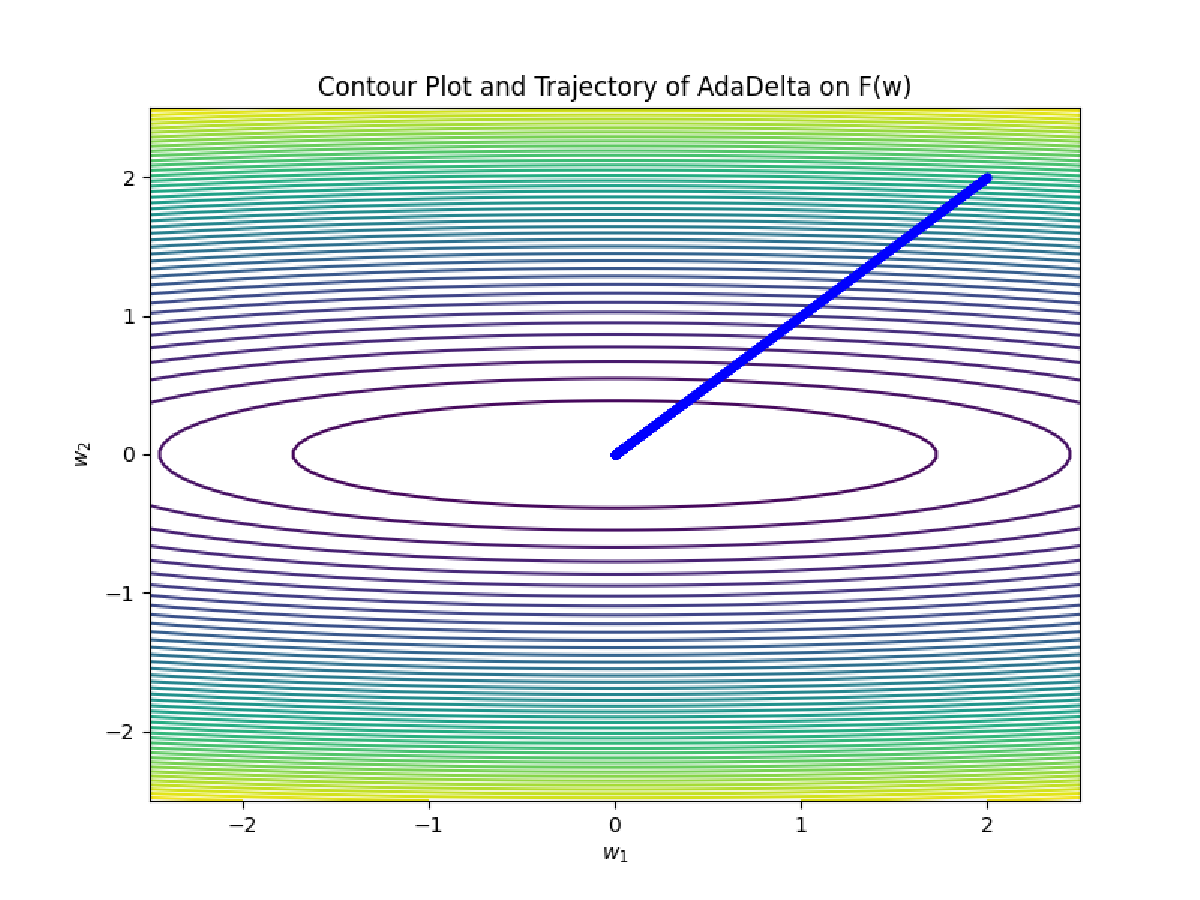
\includegraphics[width=\textwidth]{../Problem 8/ADADELTA_04.pdf}
		\caption{Initial Function with $\alpha=0.4$}
	\end{subfigure}
	\quad
	\begin{subfigure}{0.45\textwidth}
		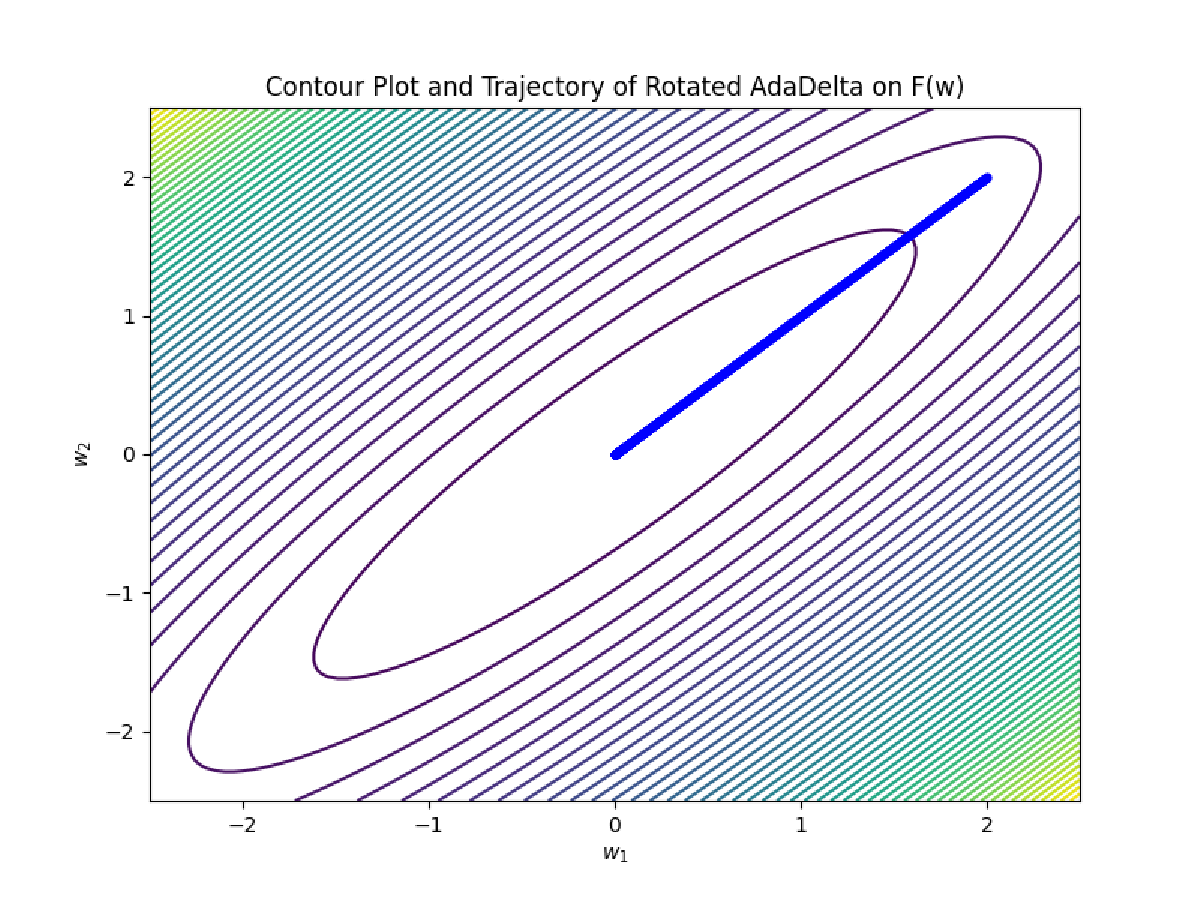
\includegraphics[width=\textwidth]{../Problem 8/ROTATED_ADADELTA.pdf}
		\caption{Rotated Function with  $\alpha=0.4$}
	\end{subfigure}
\end{figure}
\vspace{3mm}

The initial function, for learning rate $\alpha=0.4$, converges after $1236$ iterations at $\left[\num{1.21918e-05},\ \num{4.01599e-31}\right]$\\
The Rotated function, for the same learning rate, converges after $1213$ iterations at $\left[\num{3.91612e-06},\ \num{3.91612e-06}\right]$\\
